% !TEX encoding = UTF-8 Unicode
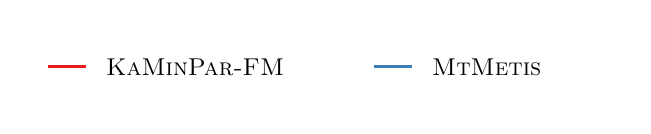
\begin{tikzpicture}[x=1pt,y=1pt]
\definecolor{fillColor}{RGB}{255,255,255}
\begin{scope}
\definecolor{fillColor}{RGB}{255,255,255}

\path[fill=fillColor] ( 55.02,238.77) rectangle (270.19,267.12);
\end{scope}
\begin{scope}
\definecolor{fillColor}{RGB}{255,255,255}

\path[fill=fillColor] ( 60.52,244.27) rectangle ( 77.87,261.62);
\end{scope}
\begin{scope}
\definecolor{drawColor}{RGB}{228,26,28}

\path[draw=drawColor,line width= 1.1pt,line join=round] ( 62.26,252.94) -- ( 76.13,252.94);
\end{scope}
\begin{scope}
\definecolor{fillColor}{RGB}{255,255,255}

\path[fill=fillColor] (178.36,244.27) rectangle (195.70,261.62);
\end{scope}
\begin{scope}
\definecolor{drawColor}{RGB}{55,126,184}

\path[draw=drawColor,line width= 1.1pt,line join=round] (180.09,252.94) -- (193.97,252.94);
\end{scope}
\begin{scope}
\definecolor{drawColor}{RGB}{0,0,0}

\node[text=drawColor,anchor=base west,inner sep=0pt, outer sep=0pt, scale=  0.88] at ( 83.37,249.91) {\textsc{KaMinPar-FM}};
\end{scope}
\begin{scope}
\definecolor{drawColor}{RGB}{0,0,0}

\node[text=drawColor,anchor=base west,inner sep=0pt, outer sep=0pt, scale=  0.88] at (201.20,249.91) {\textsc{MtMetis}};
\end{scope}
\end{tikzpicture}
